\documentclass[11pt,a4paper]{article}

\usepackage[margin=1in]{geometry}
\usepackage{graphicx}
\usepackage{amsmath,amssymb}
\usepackage{listings}
\usepackage{xcolor}
\usepackage{hyperref}

\title{Reproduction Report}
\author{MitsuhaLe}
\date{May 8, 2026}

\lstset{
	basicstyle=\ttfamily\small,
	keywordstyle=\color{blue},
	commentstyle=\color{gray},
	stringstyle=\color{teal},
	numbers=left,
	numberstyle=\tiny\color{gray},
	stepnumber=1,
	numbersep=6pt,
	showstringspaces=false,
	breaklines=true,
	frame=single
}

\begin{document}
\maketitle

\section{Overview}

I reproduced the block Newton method for nonlinear eigenvalue problems,
which was proposed by D. Kressner. The original paper is \emph{A block Newton method for nonlinear eigenvalue problems} (https://doi.org/10.1137/15M1049426). 
Overall, the algorithm is rather concise and implementation-friendly. It also exhibits local quadratic convergence.
I spent roughly one week understanding and implementing the algorithm. The code is available at \url{https://github.com/MitsuhaLe/nep-block-newton-matlab}.
During the reproduction process, I made some severe minor mistakes, which are presented in the following sections. 

It is worth noting that I also ask for help from AI tools, such as ChatGPT and Copilot.

\section{Phase 1: Understanding the Algorithm}
After reading the paper carefully, I found that the algorithm is quite straightforward. The main function has already been provided in the paper, i.e. nlevp\_newtonstep in Appendix A:

\begin{lstlisting}[language=Matlab,caption={nlevp\_newtonstep function from the original paper.},label={lst:nlevp_newtonstep}]
function [dX, dS] = nlevp_newtonstep( A, f, X, S, W, RT, RV )
% Computes the solution (dX,dS) to the linearized system in one 
% step of
% the block Newton method for a nonlinear eigenvalue problem (NLEVP).
% Input: A  - 3d-array containing the matrices A_j of the NLEVP
%        f  - handle to a function f(j,M) that returns f_j(M)
%             for any square matrix M
%        (X,S) - current iterate. S is assumed upper triangular.
%        W  - 3d-array containing the normalization matrices W_j
%        (RT,RV) - right-hand side
\end{lstlisting}

The remaining tasks were to implement algorithm 2 in the paper for setting up an initial pair $(X_0, S_0)$  
and the Armijo rule.

\section{Phase 2: Implementing the Algorithm}
My target platform was MATLAB. At first, I implemented the algorithms without a clear structure.
I only hope that the code would run and give the correct output. Unfortunately, I made quite a few mistakes in coding.
Meanwhile, I also doubted the effectiveness of the block newton method itself, since it is only a locally convergent method.
So I wasted a lot of time on debugging and trying to make the algorithm work. 

I spent an entire day working only in MATLAB. It seemed that I was still far from a correct implementation. 
Then I searched for some existing implementations online. I found a Julia implementation in \url{https://github.com/NEP-Pack}. 
There is an example of the "gun" problem, which is a standard test problem for nonlinear eigenvalue problems.
I tried to run the example, and it really worked. 
I was impressed by the performance of the code and the language Julia itself.
Then I told myself that I should try to understand the code and implement it in MATLAB. 


% \begin{figure}[h]
% 	\centering
% 	\includegraphics[width=0.7\textwidth]{figures/example.png}
% 	\caption{Example figure caption.}
% 	\label{fig:example}
% \end{figure}

\section{Phase 3: Debugging and Mistakes}
\subsection{Mistakes 1}
NEP-PACK provides the following code for the "gun" benchmark problem:
\begin{lstlisting}[caption={Example code listing.}]
nep=nep_gallery("nlevp_native_gun");
n=size(nep,1)
S=150^2*[1.0 0; 0 1]; V=[[1 0; 0 1]; zeros(n-2,2)];
(Z,X)=blocknewton(nep,S=S,X=V,logger=1,armijo_factor=0.5,maxit=20)
\end{lstlisting}
After 14 iterations, the error is 2.525942e-15.

Note the above codes call the function \verb|blocknewton|. I wanted to debug with this function, in order to inspect the intermediate outputs. However, I found all my debugging attempts failed.
I was really confused. I doubted that I was not familiar with the language Julia, which made debugging difficult for me. 
Then with the help of AI tools, I found that what I changed was the local file named \verb|method_blocknewton.jl|, 
while the code calling the function \verb|blocknewton| is calling the function in the NEP-PACK package.
This is \emph{mistake 1}. I realized that I have to integrate the function \verb|method_blocknewton| into my code.

\subsection{Mistake 2}
After fixing the above mistake, I obtained a working file named \verb|testgun.jl|.
Then I compared this implementation in Julia with my MATLAB code line by line. I found that the two codes are quite similar, except for some details. 
In MATLAB, I used some functions, such as \verb|exp, sqrt|, for matrix functions. 
However, these functions operate entrywise on matrices, which is not what I actually want.
A senior labmate told me that I should use \verb|expm, sqrtm| for matrix functions.
This is \emph{mistake 2.1}. 
Besides, I used \verb|A - 2| to denote $A - 2I$, which is also wrong and should be \verb|A - 2*eye(size(A))|. This is \emph{mistake 2.2}.

\section{Phase 4: Final Results}
I successfully implemented the block newton method in MATLAB. I tested it on the "gun" problem. It worked well but it was much slower than the Julia implementation. I used MATLAB's profiler to find the bottleneck, and it turns out that solving linear systems are the main time-consuming part.
The results are shown in the following pictures.

\begin{figure}[h]
    \centering
    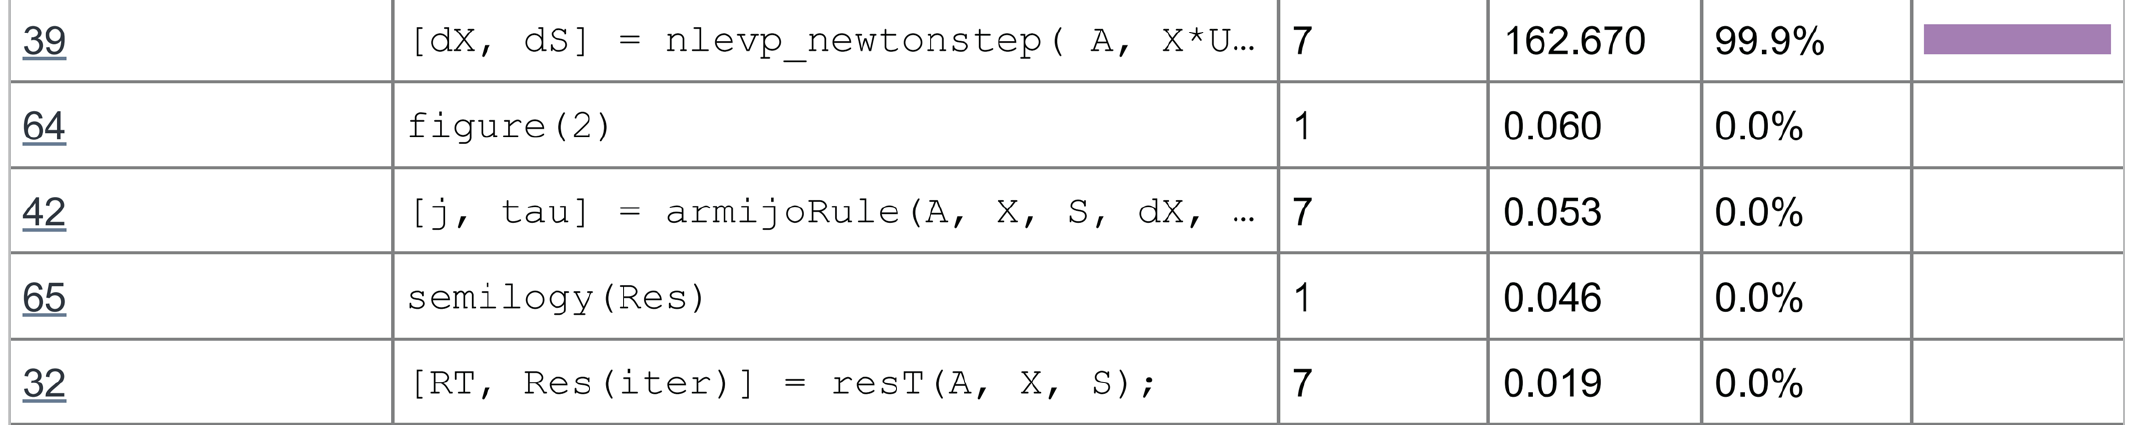
\includegraphics[width=0.7\textwidth]{profiler1.png}

    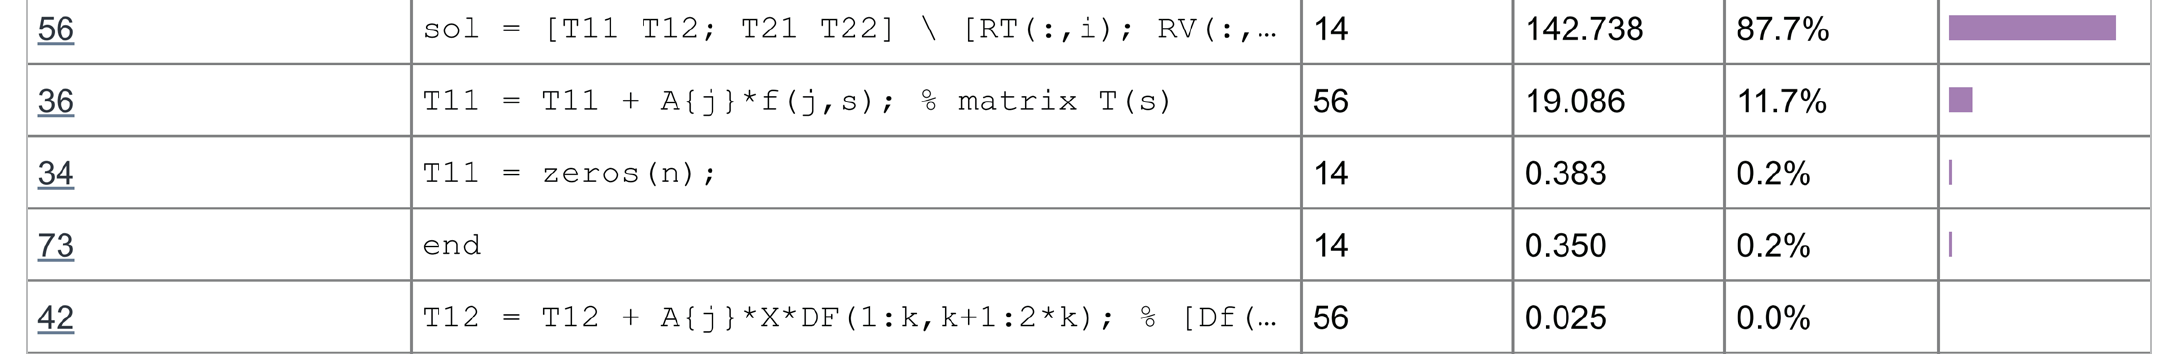
\includegraphics[width=0.7\textwidth]{profiler2.png}
    \caption{Profiler results.}
    \label{fig:example}
\end{figure}

\section{Summary and Conclusions}
I don't have much experience in reproducing papers before. This project tells me that 
reproduction studies is very meaningful. It can help me understand the algorithm deeply, and even 
give me some insights into the algorithm and the problem(here, NEP).

I need to get more coding practice, and also learn more about the language Julia. I think Julia is a very good language for scientific computing, and I may try to use it more in the future. Compared with MATLAB, Julia is more comlicated and less convenient, since its development ecosystem is less mature than MATLAB's.

Next time, I will try to avoid the mistakes I made in this project, and also try to make
my codes more concise and structured.
\end{document}
